\begin{frame}{{\em userspace} vs. {\em kernelspace}}{Systemcalls}
\begin{center}
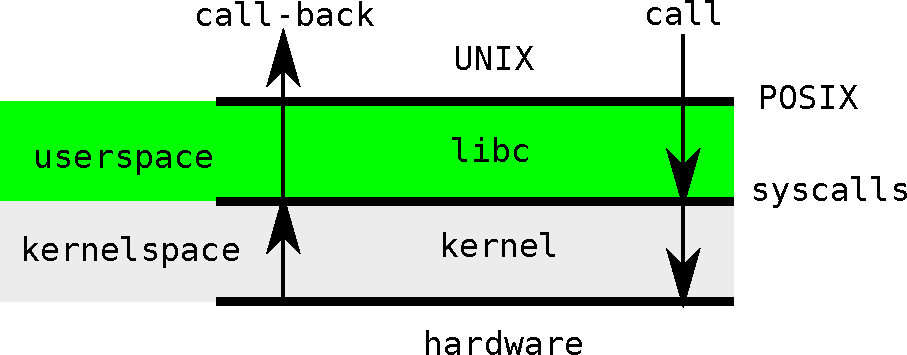
\includegraphics[width=10cm]{userspace-kernelspace.pdf}
\end{center}
\begin{description}[kernelspace]
 \item[userspace] geschützt, limitierte Zugriffsmöglichkeiten
 \item[kernelspace] ungeschützt, unlimitierte Zugriffsmöglichkeiten
\end{description}
\end{frame}

\subsection{syscalls}
\begin{frame}[fragile]{Syscall aus {\em user} Sicht }{\src{syscall-c.c}}
 \begin{lstlisting}[basicstyle=\footnotesize]
 /* write(f,void* buffer,unsigned len) */
 char s[]="Hello World\n";
         /*01234567890 */
 syscall(4,0,s,12);  /* we are in userspace */
     /*  |------------------ code for write */
 \end{lstlisting}
\end{frame}

\begin{frame}{Verzeichnisstruktur}
\dirtree{%
.1 25-modules.
.2 config.
.3 Makefile \DTcomment{for userspace}.
.2 tc \DTcomment{link to toolchain}.
.2 target \DTcomment{sshfs \targetS}.
.2 tools.
.3 modules.sh \DTcomment{script}.
.2 work.
}
\remark{Siehe auch 17-build}
\end{frame}

\subsection{Aufgaben}
\begin{frame}{Aufgaben}
 \begin{itemize}
  \item Systemcall für \host/\targetS mit \c und \cpp
 \end{itemize}
\end{frame}
